\chapter{The MOSFET: A Switch Controlled by Voltage}
\label{ch:mosfet}

Every digital chip is built from one device repeated billions of times: the \term{MOSFET}, short for metal--oxide--semiconductor field-effect transistor. If you understand this chapter, a surprising number of assessment questions become easy, including the swapped inverter and every question about ``strong'' and ``weak'' logic levels.

\section{What we want}

We want a switch with three wires. Two wires are the ends of the switch, and current flows between them when the switch is closed. The third wire controls the switch: a high voltage on it closes the switch, a low voltage opens it. Crucially, the control wire should not draw any steady current, so one switch can control many others without being drained.

The MOSFET does exactly this. Its terminals are:
\begin{itemize}
  \item the \term{gate} (G): the control input;
  \item the \term{source} (S) and \term{drain} (D): the two ends of the switch;
  \item the \term{body} (B), also called the bulk or substrate: the silicon underneath, usually tied to a fixed voltage and often not drawn.
\end{itemize}

\section{Inside an NMOS transistor}

Figure~\ref{fig:nmoscross} shows a slice through an NMOS transistor. Starting from p-type silicon (the body), two heavily doped n+ regions are formed: the source and the drain. Between them, on the surface, sits a very thin layer of insulating oxide, and on top of that the gate electrode. The distance from source to drain is the channel \term{length} $L$; the distance into the page is the channel \term{width} $W$.

\begin{figure}[h]
\centering
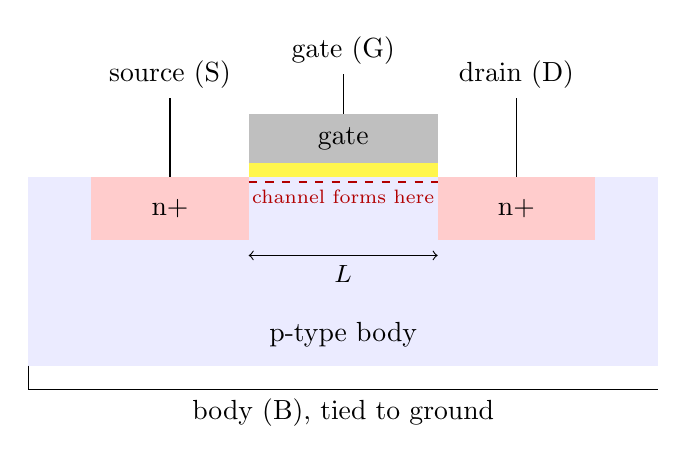
\begin{tikzpicture}[scale=1.0]
  \fill[blue!8] (0,0) rectangle (8,2.4); \node at (4,0.4) {p-type body};
  \fill[red!20] (0.8,1.6) rectangle (2.8,2.4); \node at (1.8,2.0) {n+};
  \fill[red!20] (5.2,1.6) rectangle (7.2,2.4); \node at (6.2,2.0) {n+};
  \fill[yellow!70] (2.8,2.4) rectangle (5.2,2.58);
  \fill[gray!50] (2.8,2.58) rectangle (5.2,3.2); \node at (4,2.88) {gate};
  \draw (1.8,2.4) -- (1.8,3.4) node[above]{source (S)};
  \draw (6.2,2.4) -- (6.2,3.4) node[above]{drain (D)};
  \draw (4,3.2) -- (4,3.7) node[above]{gate (G)};
  \draw (0,0) -- (0,-0.3) -- (8,-0.3); \node[below] at (4,-0.3) {body (B), tied to ground};
  \draw[<->] (2.8,1.4) -- node[below,font=\small]{$L$} (5.2,1.4);
  \draw[dashed,red!70!black,thick] (2.8,2.33) -- (5.2,2.33);
  \node[font=\scriptsize,red!70!black] at (4,2.15) {channel forms here};
\end{tikzpicture}
\caption{Cross-section of an NMOS transistor. The yellow strip under the gate is the thin insulating oxide.}
\label{fig:nmoscross}
\end{figure}

\section{How the channel forms}

With the gate at 0\,V, look at the path from source to drain: n+ silicon, then p-type body, then n+ silicon. That is two PN junctions back to back (Chapter~\ref{ch:semis}), and whichever way you push current, one of them is reverse biased. No current flows. The switch is \emph{open}.

Now raise the gate voltage. The gate, the oxide and the silicon form a capacitor. A positive gate attracts negative charge to the silicon surface just under the oxide: it pushes holes away and pulls in electrons. Once the gate voltage is high enough, electrons outnumber holes in a thin surface layer. That layer has effectively become n-type: an \term{inversion layer}, or \term{channel}. Now there is a continuous n-type path from source to drain, and current can flow. The switch is \emph{closed}.

The gate-to-source voltage needed to form the channel is the \term{threshold voltage}, $\Vt$. In modern chips it is typically 0.2 to 0.5\,V, with supply voltages around 0.7 to 1.2\,V.

\begin{bigidea}
An NMOS transistor is on when its gate is higher than its source by more than the threshold voltage: $V_{GS} > \Vtn$. The higher the gate goes above that, the more electrons fill the channel, the lower its resistance, and the more current it carries.
\end{bigidea}

\paragraph{The gate draws no steady current.} The gate sits on an insulator, so no DC current flows into it. The only current is the brief flow needed to charge or discharge the gate capacitance when its voltage changes. This is why a CMOS logic gate uses almost no power when nothing is switching, and why one gate's output can drive many other gates' inputs.

\paragraph{Which end is the source?} An NMOS transistor is physically symmetric; nothing in the silicon marks one n+ region as ``source.'' By definition, the \textbf{source of an NMOS is whichever end is at the lower voltage} (electrons flow out of the source). This sounds like a technicality, but it is the key to the ``weak 1'' later in this chapter.

\section{The PMOS transistor}

A \term{PMOS} transistor is the mirror image. It is built in n-type silicon (an \term{n-well}), with p+ source and drain regions. A channel of \emph{holes} forms when the gate is pulled sufficiently \emph{below} the source:
\[
  V_{SG} > |\Vtp| \quad \text{(gate lower than source by more than the threshold magnitude)}.
\]
The source of a PMOS is whichever end is at the \emph{higher} voltage, usually the supply $\VDD$. The n-well is tied to $\VDD$, the highest voltage, to keep its junctions reverse biased.

Because holes are about two to three times less mobile than electrons (Chapter~\ref{ch:semis}), a PMOS carries less current than an NMOS of the same size.

\section{The switch model}

For most logic design, this simple model is enough. Here $\VDD$ (logic 1) is the supply and 0\,V (logic 0) is ground.

\begin{figure}[h]
\centering
\begin{circuitikz}
  \draw (0,0) node[nmos](n){};
  \node[left] at (n.G) {G}; \node[right] at (n.D) {D}; \node[right] at (n.S) {S};
  \node at (0,-1.4) {NMOS};
  \draw (4,0) node[pmos](p){};
  \node[left] at (p.G) {G}; \node[right] at (p.S) {S}; \node[right] at (p.D) {D};
  \node at (4,-1.4) {PMOS (bubble = active low)};
\end{circuitikz}
\caption{Circuit symbols. The PMOS symbol's bubble on the gate means ``on when the gate is low.''}
\end{figure}

\begin{center}
\begin{tabular}{lll}
\toprule
 & Gate $= 1$ ($\VDD$) & Gate $= 0$ (ground) \\
\midrule
NMOS & ON (closed) & OFF (open) \\
PMOS & OFF (open) & ON (closed) \\
\bottomrule
\end{tabular}
\end{center}

\begin{remember}
NMOS: on when the gate is high. PMOS: on when the gate is low. The bubble on the PMOS symbol is a reminder: the bubble means ``inverted.''
\end{remember}

\section{How much current: regions of operation}

The switch model says only on or off. To understand speed and power we need to know how \emph{much} current flows. Define the \term{overdrive} $V_{ov} = V_{GS} - \Vt$: how far the gate is above threshold. An NMOS operates in one of three regions:

\begin{itemize}
  \item \textbf{Cutoff} ($V_{GS} < \Vt$): no channel. Ideally zero current; really a small \term{subthreshold leakage} (below).
  \item \textbf{Linear} or \textbf{triode} ($V_{GS} > \Vt$ and $V_{DS} < V_{ov}$): the channel stretches all the way from source to drain. The transistor acts like a resistor whose value the gate controls:
  \[
    I_D = \mu C_{ox}\frac{W}{L}\left(V_{ov} V_{DS} - \tfrac12 V_{DS}^2\right).
  \]
  \item \textbf{Saturation} ($V_{GS} > \Vt$ and $V_{DS} \ge V_{ov}$): near the drain, the voltage between gate and channel is too small to hold the channel open, so the channel ``pinches off.'' Raising the drain voltage further barely changes the current, which is now set by the gate:
  \[
    \boxed{I_D = \tfrac12\,\mu C_{ox}\frac{W}{L}\,(V_{GS} - \Vt)^2}
  \]
\end{itemize}

Here $\mu$ is the carrier mobility and $C_{ox}$ the gate-oxide capacitance per unit area. The product $\mu C_{ox}$ is a constant for a given manufacturing process.

\begin{figure}[h]
\centering
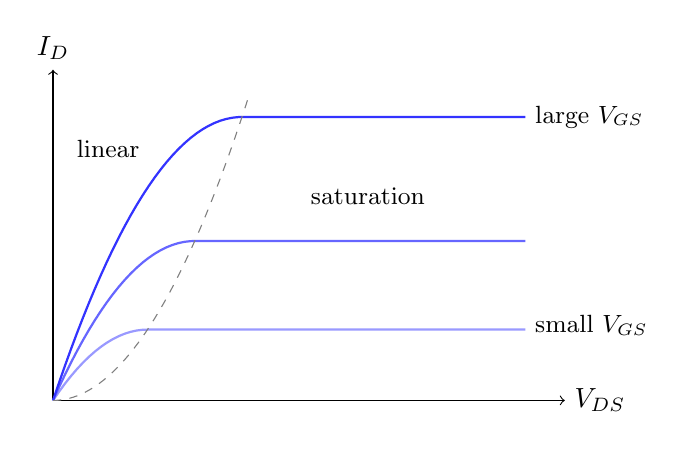
\begin{tikzpicture}[scale=1.0]
  \draw[->] (0,0) -- (6.5,0) node[right]{$V_{DS}$};
  \draw[->] (0,0) -- (0,4.2) node[above]{$I_D$};
  \foreach \v/\c in {1.2/blue!40,1.8/blue!60,2.4/blue!80} {
    \draw[thick,\c,domain=0:6,samples=80] plot (\x,{ (\x<\v) ? (\v*\x - 0.5*\x*\x)*1.25 : (0.5*\v*\v)*1.25 });
  }
  \node[right,font=\small] at (6,0.95) {small $V_{GS}$};
  \node[right,font=\small] at (6,3.6) {large $V_{GS}$};
  \draw[dashed,gray,domain=0:2.5,samples=40] plot (\x,{0.5*\x*\x*1.25});
  \node[font=\small] at (0.7,3.2) {linear};
  \node[font=\small] at (4.0,2.6) {saturation};
\end{tikzpicture}
\caption{Drain current versus drain voltage for three gate voltages. The dashed curve separates the linear region (left) from saturation (right).}
\end{figure}

What the saturation formula tells you:
\begin{itemize}
  \item \textbf{Wider is stronger}: current is proportional to $W$. Doubling the width doubles the current.
  \item \textbf{Shorter is stronger}: current is proportional to $1/L$. This is why each new manufacturing generation shrinks $L$.
  \item \textbf{More overdrive is stronger}: current grows with $(V_{GS} - \Vt)^2$. Raising the supply voltage speeds up circuits; raising the threshold slows them down.
  \item \textbf{Higher mobility is stronger}: NMOS beats PMOS of the same size.
\end{itemize}

\begin{worked}{saturation current}
An NMOS has $\mu C_{ox} = 200~\mu$A/V$^2$, $W/L = 4$, $\Vt = 0.4$\,V and $V_{GS} = 1.0$\,V, in saturation. Find $I_D$.
\[
  I_D = \tfrac12 \times 200\times10^{-6} \times 4 \times (1.0 - 0.4)^2 = 400\times10^{-6} \times 0.36 = 144~\mu\text{A}.
\]
\end{worked}

\paragraph{Real modern transistors.} The square law is a teaching model from older, longer transistors. In today's very short transistors, carriers hit their maximum velocity (velocity saturation, Chapter~\ref{ch:semis}), and current grows more like $(V_{GS} - \Vt)^{1}$ to $(V_{GS}-\Vt)^{1.3}$ than the square. Saturation current also creeps up slightly with $V_{DS}$ (\term{channel-length modulation}). The trends above still hold, and assessment questions use the simple model.

\paragraph{Subthreshold leakage.} Below threshold the current is small but not zero; it falls off \emph{exponentially} as $V_{GS}$ drops below $\Vt$, by roughly a factor of 10 for every 60 to 100\,mV at room temperature. So a transistor with a lower threshold voltage leaks exponentially more when it is ``off.'' This is the main source of leakage power (Chapter~\ref{ch:power}).

\section{Strong and weak logic levels}
\label{sec:weak1}

This section is the single most important idea for transistor-level assessment questions.

Use an NMOS as a \term{pass transistor}: its gate is held at $\VDD$ (fully on), one end is the input, and the other end drives an output node that has some capacitance (Figure~\ref{fig:passnmos}).

\begin{figure}[h]
\centering
\begin{circuitikz}
  \draw (0,0) node[nmos, rotate=-90](n){};
  \draw (n.G) -- ++(0,0.5) node[above]{gate $=\VDD$};
  \draw (n.S) -- ++(-0.8,0) node[left]{input};
  \draw (n.D) -- ++(1.0,0) coordinate(o) to[C, l=$C_{\text{load}}$] ++(0,-1.6) node[ground]{};
  \draw (o) -- ++(1.0,0) node[right]{output};
\end{circuitikz}
\caption{An NMOS pass transistor charging or discharging a load.}
\label{fig:passnmos}
\end{figure}

\paragraph{Passing a 0.} The input is 0\,V and the output starts high. The input end is the lower voltage, so it is the source, fixed at 0\,V. Then $V_{GS} = \VDD - 0 = \VDD$, comfortably above $\Vt$, for the whole discharge. The transistor stays fully on and pulls the output all the way to 0\,V. This is a \term{strong 0}.

\paragraph{Passing a 1.} The input is $\VDD$ and the output starts at 0\,V. Now the \emph{output} is the lower-voltage end, so the output is the source. As the output charges up, $V_{GS} = \VDD - V_{\text{out}}$ shrinks. When $V_{\text{out}}$ reaches $\VDD - \Vtn$, the gate is only $\Vtn$ above the source, and the transistor turns off. The output gets stuck one threshold below the supply:
\[
  V_{\text{out, max}} = \VDD - \Vtn.
\]
This is a \term{weak 1} (also called a degraded 1).

\begin{worked}{a weak 1}
$\VDD = 1.0$\,V, $\Vtn = 0.3$\,V. An NMOS pass transistor with its gate at $\VDD$ passes a 1. The output rises only to $1.0 - 0.3 = 0.7$\,V.
\end{worked}

The PMOS is the mirror image. Its source is its higher end. Passing a 1, the input (at $\VDD$) is the source, the gate is at 0, and the transistor stays fully on: a \term{strong 1}. Passing a 0, the output becomes the source; the PMOS turns off when the output falls to $|\Vtp|$, leaving a \term{weak 0}.

\begin{center}
\begin{tabular}{lll}
\toprule
 & Passes 0 & Passes 1 \\
\midrule
NMOS & strong (reaches 0\,V) & weak (stops at $\VDD - \Vtn$) \\
PMOS & weak (stops at $|\Vtp|$) & strong (reaches $\VDD$) \\
\bottomrule
\end{tabular}
\end{center}

\begin{bigidea}
NMOS is good at pulling \emph{down}; PMOS is good at pulling \emph{up}. That is why every CMOS logic gate uses NMOS transistors to connect the output to ground and PMOS transistors to connect it to the supply, and never the other way around. Chapter~\ref{ch:cmos} shows what goes wrong when you swap them.
\end{bigidea}

\paragraph{The general rule.} An NMOS whose gate is at $V_G$ can pass a voltage up to $V_G - \Vtn$, and no higher:
\[
  V_{\text{out}} = \min\left(V_{\text{in}},\; V_G - \Vtn\right).
\]
(This ignores the body effect, described below, which makes the drop slightly larger.)

\section{Chains of pass transistors}
\label{sec:passchain}

Questions often chain several pass transistors together. Two cases behave very differently.

\paragraph{Case 1: transistors in series, all gates at $\VDD$.} The threshold drop happens only \emph{once}. The first transistor passes at most $\VDD - \Vt$. The second transistor also has its gate at $\VDD$, so it too can pass up to $\VDD - \Vt$; it has no trouble passing a voltage that is already that low. The output of the chain is $\VDD - \Vt$, not $\VDD - 2\Vt$.

\paragraph{Case 2: one transistor's output drives the next transistor's gate.} Now the drops \emph{accumulate}. If node N1 is only at $\VDD - \Vt$ and it drives the gate of the next transistor, that transistor can pass only up to $(\VDD - \Vt) - \Vt$.

\begin{worked}{node voltages in a pass-transistor network}
All NMOS transistors are identical with $\Vt = 2$\,V; the supply is $\VDD = 5$\,V (an older, high-voltage process, used here to make the numbers easy to follow). Ignore the body effect.

\begin{enumerate}
  \item Transistor M1 has its gate at 5\,V and passes an input of 4\,V to node N1. \\
  $V_{N1} = \min(4,\; 5 - 2) = 3$\,V. The input is limited by the gate.
  \item Node N1 (3\,V) drives the gate of transistor M2, which passes 5\,V from the supply to node N2. \\
  $V_{N2} = \min(5,\; 3 - 2) = 1$\,V.
  \item Node N2 (1\,V) drives the gate of transistor M3. Since $1~\text{V} < \Vt = 2$\,V, M3 is off and passes nothing.
  \item Instead, suppose M1 is followed by M4, in series, also with its gate at 5\,V. The output of M4 is $\min(3,\; 5-2) = 3$\,V: no extra drop.
\end{enumerate}
\end{worked}

\begin{onoa}
A reported question asked for the voltages at several nodes of a network of identical NMOS transistors with $\VDD = 5$\,V, $\Vt = 2$\,V and an input of 4\,V. Without the original diagram, the method above is what such questions test: at each node apply $V_{\text{out}} = \min(V_{\text{in}}, V_G - \Vt)$, notice whether a gate is driven by the full supply or by an already-degraded node, and check whether any transistor's gate falls below threshold.
\end{onoa}

\section{The body effect}

So far we assumed the threshold voltage is fixed. In fact, an NMOS's threshold \emph{increases} when its source is above its body. In a pass transistor passing a 1, the source rises toward $\VDD$ while the body stays at ground, so $\Vt$ grows as the output rises, making the weak 1 even weaker. Transistors stacked in series (where the upper ones have sources above ground) are also slightly weakened. For assessment questions, it is enough to know the direction: \textbf{a source above the body raises $\Vt$}.

\section{Sizing transistors}
\label{sec:sizing}

Because current is proportional to $\mu\,W/L$, a designer chooses $W$ (and sometimes $L$) to set each transistor's strength. To make a PMOS deliver the same current as an NMOS, it must make up for its lower mobility with extra width:
\[
  \frac{(W/L)_p}{(W/L)_n} = \frac{\mu_n}{\mu_p} \approx 2 \text{ to } 3.
\]

\begin{worked}{equal saturation currents}
In a process where $\mu_n = 2.5\,\mu_p$, the NMOS in an inverter is 1\,$\mu$m wide. Both have the same length. How wide should the PMOS be so both deliver the same current?

$W_p = 2.5 \times 1 = 2.5~\mu$m.
\end{worked}

The trade-off: a wider transistor is stronger, but its gate has more capacitance, so whatever drives \emph{it} has a bigger load and becomes slower. Sizing is a balance (Chapter~\ref{ch:delay}).

\section{Transistor capacitance}

A transistor's gate is a capacitor: gate on one side, channel on the other, oxide between. Its capacitance is roughly
\[
  C_g = C_{ox}\,W\,L.
\]
The source and drain regions also have capacitance to the body, called \term{diffusion capacitance}. When a gate's output switches, it must charge the input capacitance of every gate it drives, the wires in between, and its own diffusion capacitance.

\section{Threshold voltage as a design knob}

Chip processes usually offer several transistor flavors with different thresholds:
\begin{itemize}
  \item \textbf{Low-$\Vt$} transistors: more overdrive, so faster, but they leak exponentially more when off.
  \item \textbf{High-$\Vt$} transistors: slower but with far less leakage.
\end{itemize}
Designers use fast low-$\Vt$ transistors only on the few paths that limit speed, and high-$\Vt$ transistors everywhere else to save leakage power. Temperature also changes $\Vt$: it \emph{decreases} as the chip heats up (Chapter~\ref{ch:pvt}).

\section{Modern transistor shapes}

As $L$ shrank to tens of nanometers, a gate sitting only on top of the channel could no longer fully control it, and leakage grew. Two newer structures fix this by wrapping the gate around more of the channel:
\begin{itemize}
  \item \term{FinFET}: the channel is a thin vertical fin, and the gate wraps over three sides.
  \item \term{Gate-all-around} (GAA) or \term{nanosheet}: the channel is a stack of thin horizontal sheets, each surrounded by the gate on all four sides.
\end{itemize}
More gate control means the transistor turns off more completely, which reduces leakage. The basic switch behavior in this chapter is unchanged.

\section{Summary}

\begin{itemize}
  \item A MOSFET is a voltage-controlled switch: gate controls whether current flows between source and drain. The gate draws no DC current.
  \item NMOS: on when $V_{GS} > \Vtn$ (gate high). PMOS: on when $V_{SG} > |\Vtp|$ (gate low).
  \item NMOS source is its lower-voltage end; PMOS source is its higher-voltage end.
  \item Saturation current: $I_D = \tfrac12\mu C_{ox}(W/L)(V_{GS}-\Vt)^2$. Wider, shorter, more overdrive and higher mobility all mean more current.
  \item NMOS passes a strong 0 and a weak 1 ($\VDD - \Vtn$). PMOS passes a strong 1 and a weak 0 ($|\Vtp|$).
  \item Pass-transistor rule: $V_{\text{out}} = \min(V_{\text{in}}, V_G - \Vt)$. Drops do not add in a series chain with full gates; they do add when degraded nodes drive gates.
  \item PMOS is made about 2--3 times wider than NMOS for equal current.
  \item Lower $\Vt$ means faster but exponentially leakier.
\end{itemize}

\section{Exercises}

\begin{enumerate}
  \item An NMOS has $V_{GS} = 0.2$\,V and $\Vtn = 0.35$\,V. Is it on or off?
  \item A PMOS has its source at 1.0\,V, its gate at 0\,V, and $|\Vtp| = 0.3$\,V. Is it on or off?
  \item An NMOS pass transistor with its gate at $\VDD = 1.2$\,V passes a 1. If $\Vtn = 0.4$\,V, what is the highest voltage the output reaches?
  \item A PMOS pass transistor with its gate at 0\,V passes a 0. If $|\Vtp| = 0.35$\,V, what is the lowest voltage the output reaches?
  \item An NMOS in saturation has $\mu C_{ox}(W/L) = 1$\,mA/V$^2$ and $V_{GS} - \Vt = 0.5$\,V. Find $I_D$. What happens to $I_D$ if $W$ doubles?
  \item Two NMOS transistors are in series, both gates at $\VDD = 1$\,V, $\Vt = 0.3$\,V. The input is 1\,V. What is the output: 0.7\,V or 0.4\,V?
  \item An NMOS has its gate driven by a node at 0.7\,V and passes a 1.0\,V input. With $\Vt = 0.3$\,V, what is the output?
  \item In a process with $\mu_n/\mu_p = 2$, an NMOS is 0.2\,$\mu$m wide. How wide should a same-length PMOS be for equal current?
  \item Why does a MOSFET's gate draw no DC current?
  \item What is the trade-off between low-$\Vt$ and high-$\Vt$ transistors?
\end{enumerate}

\subsection*{Answers}
\begin{enumerate}
  \item Off (below threshold), apart from a small subthreshold leakage.
  \item On: $V_{SG} = 1.0 - 0 = 1.0~\text{V} > 0.3$\,V.
  \item $1.2 - 0.4 = 0.8$\,V.
  \item $0.35$\,V.
  \item $I_D = \tfrac12 \times 1\times10^{-3} \times 0.25 = 125~\mu$A. Doubling $W$ doubles it to 250\,$\mu$A.
  \item 0.7\,V. Both gates are at the full supply, so only one threshold drop occurs.
  \item $\min(1.0,\; 0.7 - 0.3) = 0.4$\,V.
  \item 0.4\,$\mu$m.
  \item The gate is separated from the channel by an insulating oxide, so the gate is a capacitor: current flows only briefly while its voltage changes.
  \item Low-$\Vt$ is faster (more overdrive) but leaks exponentially more; high-$\Vt$ is slower but leaks far less.
\end{enumerate}
